% !TEX root = main.tex

\section{简介} % ch1
图~\ref{fig:venn}反映了\newterm{深度学习}与其他几个常见概念之间的关系。
传统的\newterm{机器学习}(如决策树、SVM、随机森林等)常需要人工提取特征,这一步经常涉及到\newterm{特征工程}(feature engineering),如果特征没有进行一定处理,直接丢进去让其学习,往往会产生非常糟糕的结果。在一种表示下可能可以对数据进行线性二分,而另一种表示下则没有办法。
因此,为了避免对特征的强依赖性,一种方法是利用机器学习来学习\textbf{表示(representation)本身},再将新的表示送入到后面的学习器中让它学习\textbf{表示到输出的映射},此即\newterm{表示学习}。
再到后来,深度学习则更加将这种思想发扬光大,表示学习只能学习到\textbf{浅层简单的特征},那深度学习则尝试去学习\textbf{深层复杂的特征}。

\bigskip
\begin{tcolorbox}
事实上现在\newterm{图神经网络}(GNN)也是遵循这样的发展过程,最开始尝试在图上做机器学习\cite{yao:graph_ml_2009,li:distributed_2013,gemulla:mf_2011};然后又开始在图上以各种随机游走的方式做图表示学习-图嵌入(embedding)\cite{perozzi:deepwalk_2014,grover:node2vec_2016};后来发现图嵌入能够获得的特征依然太浅层了,因此现在更多则采用图神经网络\cite{kipf:gcn_2017,hamilton:graphsage_2017,li:gated_2016,velickovic:gat_2018}的方式来做图相关的工作。
\end{tcolorbox}

\begin{figure}[H]
\centering
\begin{tabular}{cc}
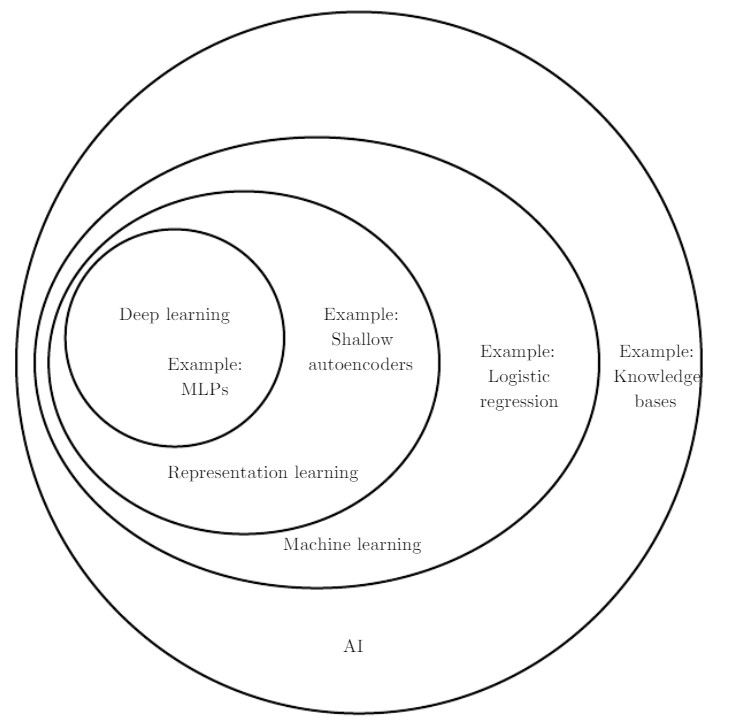
\includegraphics[width=0.5\linewidth]{fig/dl_venn.jpg}
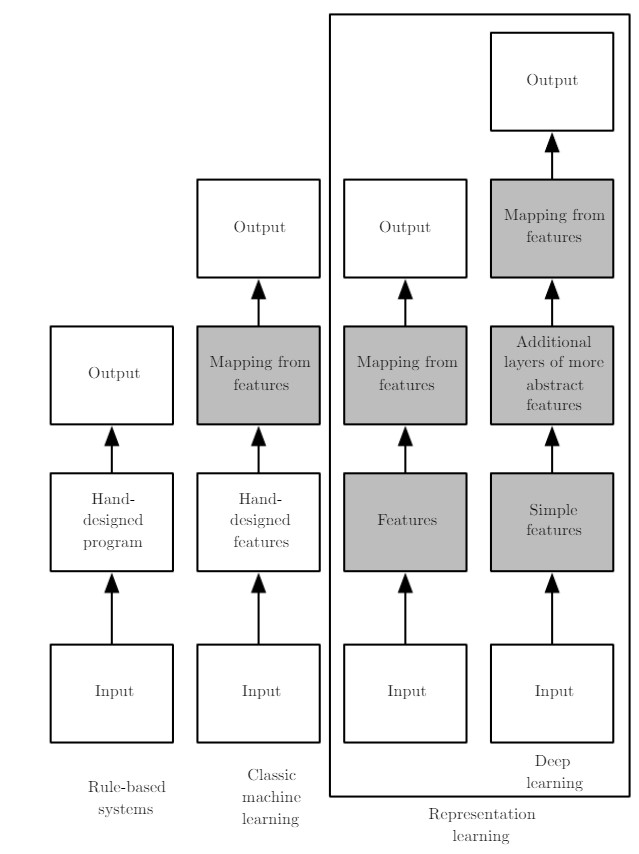
\includegraphics[width=0.5\linewidth]{fig/dl_flowchart.jpg}
\end{tabular}
\caption{深度学习Venn图}
\label{fig:venn}
\end{figure}

深度学习在发展过程中也起过几个名字:在1940年代到1960年代被称为\newterm{控制论}(cybernetics),之后\\
1980到1990年代则被称为\newterm{连接主义}(connectionism),而后从2006年到现在才被称为\newterm{深度学习}。2018年的图灵奖正式颁发给深度学习三巨头---Geoffrey Hinton,Yoshua Bengio和Yann LeCun,也奠定了深度学习在学术界的历史地位。

\bigskip
\begin{tcolorbox}
我也一直在思考是什么造成了深度学习在2010年代的兴起,使得如今我们快速进入软件2.0时代\cite{olukotun:software2_2018}。
总结来讲有以下几点:
\begin{itemize}
    \item \textbf{数据}:我们每天产生的数据量越来越多,能够处理的数据量越来越大,名副其实地进入了大数据时代。
    其中的一些数据经过处理能够变得很干净,2010年拥有大量标注图片的数据集ImageNet就是这样的例子,它的提出使得有监督学习迎来了一波兴起。
    \item \textbf{算法}:我们有更多更优秀的模型,从AlexNet的dropout,再到后来ResNet的残差模块。
    ImageNet的发展历程,也是深度学习算法/模型改进和发展的历程。
    \item \textbf{软件系统}:早年的深度学习框架Caffe、Theano、MXNet等使得研究人员可以方便地编写神经网络模型,而2015年前后诞生的TensorFlow和PyTorch则是成为了现在深度学习框架的主流范式,程序员不需知道底层的实施细节,只用“调库”和“调参”也可以实现很高效的模型,这些软件系统的诞生极大程度推动了深度学习的遍地开花。
    再到现在XLA和TVM等深度学习编译器的出现,更是进一步解放程序员,使上层模型可以方便快捷地部署到后端不同硬件平台上。
    \item \textbf{硬件}:GPU为深度学习做出了不可磨灭的贡献,没有GPGPU的发展,很多深度学习任务根本没有办法完成。
    现在的TPU及各种神经网络加速器也都是在拓宽这一层面,以进一步提升深度学习的能力。
\end{itemize}
上面提到的这几点都不可或缺,它们共同造就了整个深度学习栈,从而带来现在深度学习的繁荣。
\end{tcolorbox}